\documentclass[11pt]{beamer}

%\setbeamertemplate{caption}[numbered]
\usepackage{lmodern}
\usepackage[numbers]{natbib}
% Package to include pdf
\usepackage{pdfpages}
% Package to include pdf
\usepackage{hyperref}
\usepackage{graphicx}
\usepackage{float}
\usepackage{cutwin}
\usepackage{pdfpages}
\usepackage{hyperref}
\usepackage{tikz}
\usepackage{cutwin}
\usepackage{lipsum}
\usepackage{bm}
\usepackage{adjustbox}
\usepackage{showexpl}
\usepackage[skins,listings,raster]{tcolorbox}
% Packages for creating nice looking table
\usepackage{booktabs}
\newcommand{\ra}[1]{\renewcommand{\arraystretch}{#1}}
\usepackage{multirow}
\usepackage{multicol}
% Packages for creating nice looking table

\usetikzlibrary{arrows.meta, calc, quotes, tikzmark}
\tikzstyle{block}=[draw opacity=0.7,line width=1.4cm]

\usepackage{subcaption}
\usepackage{blindtext}
%% Add listing for brogrammer
\usepackage{listings, lstautogobble}
\usepackage{color}

% \usepackage{minted}
\definecolor{lightgrey}{rgb}{0.9,0.9,0.9}
\definecolor{darkgreen}{rgb}{0,0.6,0}

\definecolor{MS_Blue}{rgb}{0,.47843,0.8}
\definecolor{MS_Green}{rgb}{0.415686, 0.6, 0.333}

% Draw folders and files structure
% \documentclass[tikz,border=5mm]{standalone}

% \usepackage[edges]{forest}

% \definecolor{foldercolor}{RGB}{124,166,198}

% \definecolor{folderbg}{RGB}{124,166,198}
% \definecolor{folderborder}{RGB}{110,144,169}

% \def\Size{4pt}
% \tikzset{
%   folder/.pic={
%     \filldraw[draw=folderborder,top color=folderbg!50,bottom color=folderbg]
%       (-1.05*\Size,0.2\Size+5pt) rectangle ++(.75*\Size,-0.2\Size-5pt);  
%     \filldraw[draw=folderborder,top color=folderbg!50,bottom color=folderbg]
%       (-1.15*\Size,-\Size) rectangle (1.15*\Size,\Size);
%   }
% }

% \forestset{is file/.style={edge path'/.expanded={%
%         ([xshift=\forestregister{folder indent}]!u.parent anchor) |- (.child anchor)},
%         inner sep=1pt},
%     this folder size/.style={edge path'/.expanded={%
%         ([xshift=\forestregister{folder indent}]!u.parent anchor) |- (.child anchor) pic[solid]{folder=#1}}, inner ysep=0.6*#1},
%     folder tree indent/.style={before computing xy={l=#1}},
%     folder icons/.style={folder, this folder size=#1, folder tree indent=3*#1},
%     folder icons/.default={12pt},
% }
% Draw folders and files structure

% lstdefinelanguage{TeX}
% {
	
% }
\lstset{
	language=[LaTeX]TeX,
	texcsstyle=*\bf\color{MS_Blue},
	numbers=left,
	numberstyle=\tiny,
	breaklines=true,
	keywordstyle=\color{darkgreen}\bfseries\tiny,
	commentstyle=\color{MS_Green}\bfseries\tiny,
	otherkeywords = {subsection, subsubsection},
	% otherkeywords={$, \{, \}, \[, \], \\usepackage\{aa\}},
	frame=single,
	tabsize=2,
	backgroundcolor=\color{lightgrey},
	morekeywords = {document},
	basicstyle = \ttfamily\tiny,
	autogobble = true
}

%% Add listing for brogrammer

\usepackage[style=british]{csquotes}

\def\signed #1{{\leavevmode\unskip\nobreak\hfil\penalty50\hskip1em
		\hbox{}\nobreak\hfill #1%
		\parfillskip=0pt \finalhyphendemerits=0 \endgraf}}

\newsavebox\mybox
\newenvironment{aquote}[1]
{\savebox\mybox{#1}\begin{quote}\openautoquote\hspace*{-.7ex}}
	{\unskip\closeautoquote\vspace*{1mm}\signed{\usebox\mybox}\end{quote}}

\usepackage[absolute,overlay]{textpos}
  \setlength{\TPHorizModule}{1mm}
  \setlength{\TPVertModule}{1mm}

\usetikzlibrary{quotes, arrows.meta}

\usetheme{cambridge}
\setbeamertemplate{caption}[numbered]
% \usetheme{Boadilla}
\title{How to use \LaTeX}
\author{Daoming Dong \& Youchao Wang}
\institute{CMMPE, Engineering, University of Cambridge}
\date{April 20, 2019}
\begin{document}

\begin{frame}
	\titlepage
\end{frame}

\begin{frame}
	\frametitle{Why \LaTeX\ ?}
	An extremely good philosophical question.
	
	\begin{itemize}
		\item Microsoft Office Word and PowerPoint are boring.
		\item \LaTeX\ is elegant, charming, or whatever...
		\item Excellent for mathematical typesetting.
		\item Powerful, lots and lots of power for you to extend it, be it theses, papers, slides (using Beamer), spreadsheets...
		\item Free and portable, supported by most OS platforms.
	\end{itemize}

\end{frame}

\begin{frame}
\frametitle{What \LaTeX \ can do}

\begin{itemize}
	\item Write scientific papers
	\item Write theses
	\item Typeset books and publications
	\item Write typeset letters
	\item Play around with mathematical formulae
	\item Make presentation slides
	\item Beautify your CV
	\item and many more
\end{itemize}

\end{frame}

\begin{frame}
	\frametitle{Useful resources}

	Books list
	 \begin{columns}
		\column{0.5\textwidth}
		\centering
		\begin{figure}
			
\includegraphics[width=.5\linewidth]{Figures/BeginnersGuide.jpg}
			\caption{\LaTeX \ Beginner's Guide}
		\end{figure}
		\column{0.5\textwidth}
		\centering
		\begin{figure}
			
\includegraphics[width=.5\linewidth]{Figures/Lamport.jpg}
			\caption{\LaTeX: A Document Preparation System: User's Guide and Reference Manual}
		\end{figure}
	\end{columns}
\end{frame}

\begin{frame}
	\frametitle{Useful resources}

	Learn \LaTeX \ in one video : https://www.youtube.com/watch?v=VhmkLrOjLsw
	
	\bigskip
	
	Mr Daoming Dong is also a good resource. He is nice and helpful.
	
	Zhihu: @DDMichael

\end{frame}

\begin{frame}
	\frametitle{A brief history}

	In the mid 1970s, Donald Knuth, a Stanford CS geek and the academic world equivalent of Martin (the author of GOT), developed \TeX \ in SAIL to typeset his "The Art of Computer Programming" (TAOCP). First public release in 1978. He reimplemented it in Pascal in the mid 80s (WEB, literate programming).  Leslie Lamport, the genius, wrote \LaTeX \ in early 80s by porting the orginal \TeX. 
	
	\bigskip
	
	What is the relationship between \TeX \xspace and \LaTeX? 
	
	\LaTeX \ uses the \TeX \ typesetting programme to compile and generate its output. \LaTeX \ focuses on the content while \TeX \ is the main programme for setting up the layout.

\end{frame}

\begin{frame}
	\frametitle{\LaTeX version}
	
	The first \LaTeX\xspace version available is 2.09 (strange number and strange version control). Later in 1994, \LaTeXe\xspace replaced the old version, and remained ever since. \LaTeX \ 3 is a long-term research project, which started from the 1990s.
	
\end{frame}

\begin{frame}
	\frametitle{How to pronounce \LaTeX\ ?}
	
	First and foremost, the pronunciation of \LaTeX. According to the father of \TeX:
	
	\begin{aquote}{Donald Knuth}
		English words like `technology' stem from a Greek root beginning with the letters $\tau \epsilon \chi$...; and this same Greek word means art as well as technology. Hence the name TeX, which is an uppercase form of $\tau \epsilon \chi$.

		Insiders pronounce the $\chi$ of TeX as a Greek chi, not as an `x', so that TeX rhymes with the word blecchhh. It's the `ch' sound in Scottish words like loch or German words like ach; it's a Spanish `j' and a Russian `kh'. When you say it correctly to your computer, the terminal may become slightly moist.  
	\end{aquote}

\end{frame}

\begin{frame}
\frametitle{How to pronounce \LaTeX\ ?}
	
	Another quote from the father of \LaTeX:
	\begin{aquote}{Leslie Lamport}
		One of the hardest things about LaTeX is deciding how to pronounce it.This is also one of the few things I'm not going to tell you about LaTeX, since pronunciation is best determined by usage, not fiat. TeX is usually pronounced teck, making lah-teck, and lay-teck the logical choices; but language is not always logical, so lay-tecks is also possible.
	\end{aquote}

\end{frame}

\begin{frame}
	\frametitle{Installation}
	
	We would highly recommend the following \LaTeX \ distributions.
	
	\begin{itemize}
		\item For Windows users
			\begin{itemize}
				\item TeX Live
				\item MiKTeX
			\end{itemize}
		\item For MacOS users
			\begin{itemize}
				\item TeX Live
				\item MacTeX
			\end{itemize}
	\end{itemize}

	Note that the TeX Live distribution contains yearly updates, and the update installation must be done manually.

\end{frame}

\begin{frame}
\frametitle{Editors}

	There are in fact numerous ways for you to write up a \LaTeX \ document.

	\begin{itemize}
		\item TeXStudio \textbf{(behold, the beamer template we used for this tutorial cannot be built using this editor)}
		\item TeXShop
		\item Notepad \ Notepad++
		\item Sublime
		\item Visual Studio Code
		\item Vi / Vim
		\item \emph{Word} !!!
		\item Overleaf (the online editor)
	\end{itemize}

	In fact, any plain-text editor shall suffice.

\end{frame}


\begin{frame}
	\frametitle{How to use}
	
	\emph{We have to remind you that learning \LaTeX \ (might be) very hard}
	
	\begin{figure}
		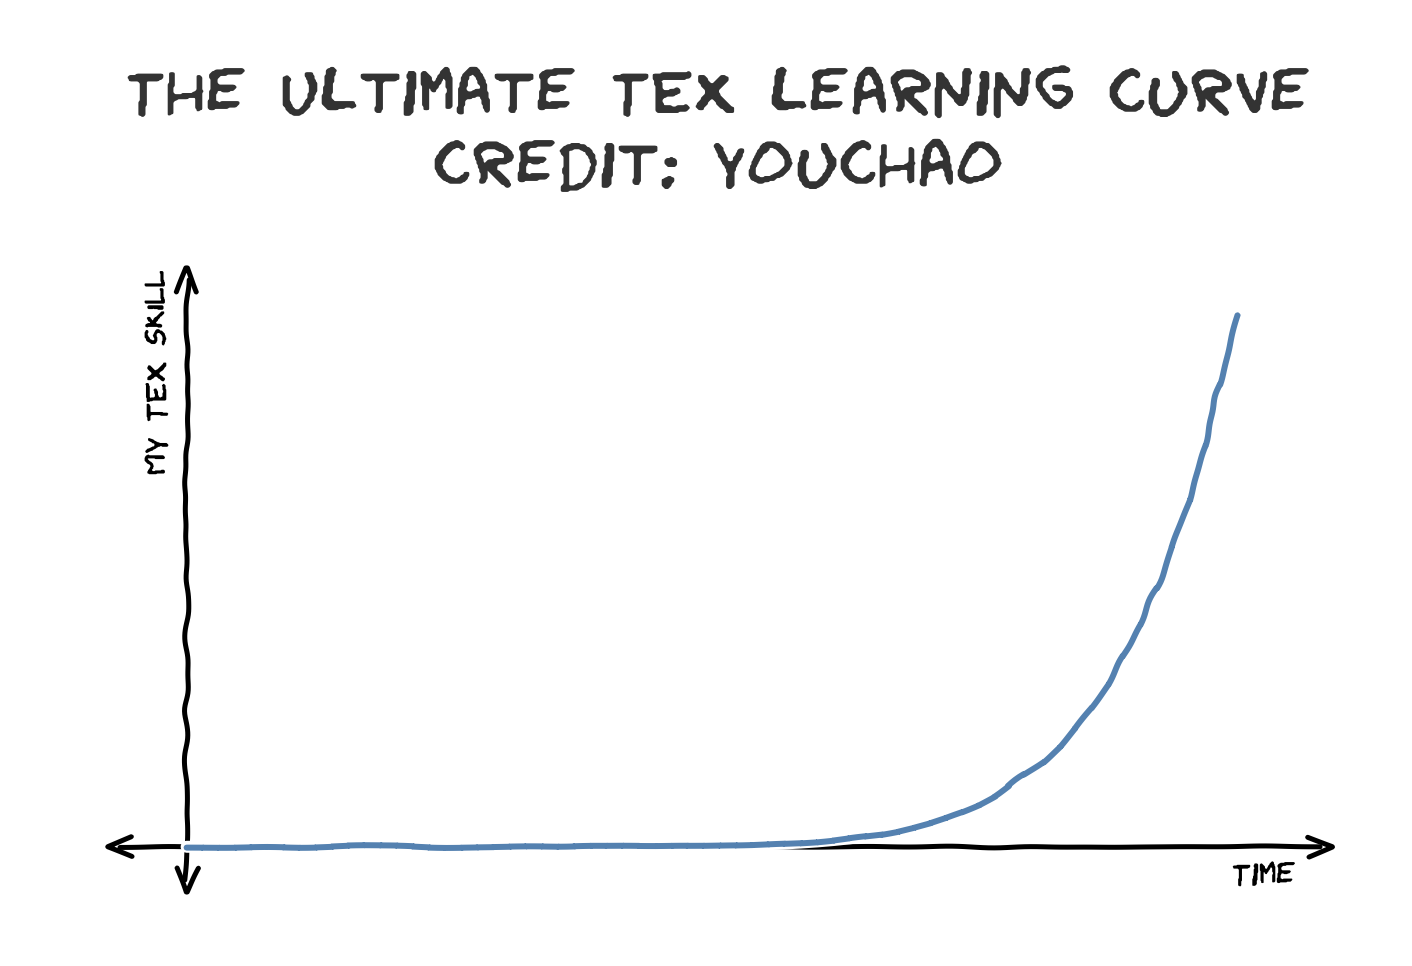
\includegraphics[width=.7\linewidth]{Figures/Curve.png}
	\end{figure}

\end{frame}

\begin{frame}
	\frametitle{How to use}
	
	\emph{We have to remind you that learning \LaTeX \  (might be) very hard  \footnotemark}
	\begin{columns}
		\tikzset{box/.style={inner xsep=0pt}}
		
		\column{0.4\textwidth}
		\raggedright
		Newbie \tikzmark{N}

		\column{0.3\textwidth}
		\raggedleft
		\tikzmark{g} Give up
	\end{columns}

	\begin{columns}
		\column{0.4\textwidth}
		
		\column{0.3\textwidth}
		\raggedleft
		%no idea how i plotted "give up" and "master", as being so far apart...
		% thankfully now i know
		
		\tikzmark{mark} Master

	\end{columns}

 	
\begin{tikzpicture}[overlay,remember picture]
		\draw[very thick, -Stealth]		($({pic cs:N})+(0ex,1ex)$)
		to [bend right, sloped, "USUALLY"]		($({pic cs:g})+(6pt,-3pt)$);
	\end{tikzpicture}
	
	 
\begin{tikzpicture}[overlay,remember picture]
		\draw[very thick, -Stealth]		($({pic cs:N})+(0pt,1ex)$)
		to [bend right,  "WANT THIS"]		($({pic cs:mark})+(6pt,-6pt)$);
	\end{tikzpicture}
	
	\footnotetext{These arrows are plotted using a package called tikz}
	
\end{frame}

\begin{frame}
	\frametitle{Some common knowledge}
	
	Since \LaTeX \ is a package implemented in the \TeX \ \textbf{typesetting language}, we should consider the \TeX \ input syntax when use it.
	
	\bigskip
	
	\TeX \ reads *.tex files and with lots of interesting background procedures, outputs *.pdf files. 
	
\end{frame}

\begin{frame}
	\frametitle{Some common knowledge}
	
	\begin{itemize}
		\item The effect of typing multiple spaces is the same as one space.
		\item The effect of typing multiple line feeds is the same as one line break.
		\item If you don't know how and when to use $\backslash$ (backslash), \textbf{then you are doomed}.
		\item Be aware of the use of \textbackslash xpace and whatever that follows the backslash after the  \textasciitilde mark, e.g., \textasciitilde \textbackslash ref.
		\item \textbackslash(white space), this forces normal space, \textbackslash @, this indicates that the next punctuation ends the sentence. Try out the differences by yourselves.
	\end{itemize}
	
\end{frame}

\begin{frame}[containsverbatim]
	\frametitle{Some common knowledge}

	\begin{itemize}
		\item Special meta characters as part of the \TeX \  language syntax:
		\begin{itemize}
			\item \# \ \$ \ \% \ \^ \ \& \ \_ \ \{ \} \ \textasciitilde \  \textbackslash
		\end{itemize}
		\item To use them you have to do the following
			\begin{verbatim}
			\# \$ \% \^ \& \_ \{ \} \textasciitilde \textbackslash
			\end{verbatim}
	\end{itemize}

\end{frame}

\begin{frame}[containsverbatim]
	\frametitle{Changing fonts and styles}
	
	You may either use (1) lexical declarations or (2) commands. \textit{\footnotesize Contents are referenced from the slides for a course held at the Computer Lab, Cambridge.}
	\begin{columns}
		\column{0.2\textwidth}
		\raggedleft
			\begin{verbatim}
			\mdseries
			\bfseries
			\rmfamily
			\sffamily
			\ttfamily
			\upshape
			\itshape
			\slshape
			\scshape
			\normalfont
			\end{verbatim}
		\column{0.3\textwidth}
			\begin{verbatim}
			\textmd{text}
			\textbf{text}
			\textrm{text}
			\textsf{text}
			\texttt{text}
			\textup{text}
			\textit{text}
			\textsl{text}
			\textsc{text}
			\textnormal{text}
			\end{verbatim}
			
		\column{0.3\textwidth}
			\bigskip
			\\
			\textmd{Medium series}\\
			\textbf{Boldface series}\\
			\textrm{Roman family}\\
			\textsf{Sans-serif family}\\
			\texttt{Typewriter family}\\
			\textup{Upright shape}\\
			\textit{Italic shape}\\
			\textsl{Slanted shape}\\
			\textsc{Small caps shape}\\
			\textnormal{Normal style}
	\end{columns}
\end{frame}


\begin{frame}[containsverbatim]
\frametitle{How to use dashes}

There are, in fact, \textbf{en dashes}, \textbf{em dashes}, \textbf{hyphens} and \textbf{minus signs}.

\bigskip

\centering
\verb|-| corresponds to - hyphen\\
\verb|--| corresponds to -- en dash\\
\verb|---| corresponds to --- em dash\\
\verb|$-$| corresponds to $-$ minus sign

\bigskip

\raggedright
For example, line-breaks (\textit{hyphen}), Figures 1--4 (\textit{en dash}), people---like me---love to use \LaTeX. 

In terms of how to properly use them, try searching the internet for answers. \textbf{Metaphysics} it is.

\end{frame}

\begin{frame}
\frametitle{How to use quotation marks}

One of the (out of many) mistakes that you will definitely make throughout your \LaTeX \ journey is the use of quotation marks.

Unlike Word, \TeX \ uses single quotation mark (') and the grave accent (`) to encode the differences.

\bigskip

\centering
\' \ corresponds to ' left quote\\
\` \ corresponds to ` right quote\\
\' \ \' \ corresponds to '' left double\\
\` \ \` \ corresponds to `` right double

\bigskip

\raggedright

\end{frame}



% \begin{frame}
% 	\frametitle{Directory structure}
% \begin{forest}
%   for tree={
%     font=\ttfamily,
%     grow'=0,
%     child anchor=west,
%     parent anchor=south,
%     anchor=west,
%     calign=first,
%     inner xsep=7pt,
%     edge path={
%       \noexpand\path [draw, \forestoption{edge}]
%       (!u.south west) +(7.5pt,0) |- (.child anchor) pic {folder} \forestoption{edge label};
%     },
%     before typesetting nodes={
%       if n=1
%         {insert before={[,phantom]}}
%         {}
%     },
%     fit=band,
%     before computing xy={l=15pt},
%   }  
% [TexFolder
%   [config
%   ]
%   [lib
%     [Access.pdf
%     ]
%     [Plugin
%     ]
%   ]
%   [templates
%   ]
%   [tests
%   ]
% ]
% \end{forest}
% \end{frame}

\begin{frame}[containsverbatim]
	\frametitle{Starting a report and title page}
	
	 \begin{columns}
		\column{0.5\textwidth}
		\centering
		\begin{minipage}{0.9\textwidth}
			\begin{lstlisting}
\documentclass{article}
\begin{document}
\begin{titlepage}
	\begin{center}
		\line(1,0){300}\\
		[0.25in]
		\huge{\textbf{ CSSA \LaTeX\ Notes}}\\
		[2mm]
		\line(1,0){200}\\
		[1.5cm]
		\textsc{\LARGE University of Cambridge}\\
		\textsc{\LARGE Using \LaTeX\ to Write a Simple Report}\\
		[8cm]
	\end{center}
	\begin{flushright}
		\textsc{\large CSSA. \\ A Latex User\\
		20th Apr 2019}
	\end{flushright}
\end{titlepage}
\end{document}
			\end{lstlisting}
		\end{minipage}
			\column{0.5\textwidth}
			\begin{minipage}{0.98\textwidth}
				\begin{figure}
					\frame{
\includegraphics[page = 1, width=0.8\textwidth]{CodeSnippets/StartingAReport.pdf}}
				\end{figure}
			\end{minipage}
\end{columns}

\end{frame}


\begin{frame}[containsverbatim]
	\frametitle{Sections}
	 \begin{columns}
		\column{0.5\textwidth}
		\centering
		\begin{minipage}{0.9\textwidth}
			\begin{lstlisting}
\section{Introduction} 
This is the first line of the report. This report will show you how to use \LaTeX\\\
% Text holder: show one paragraph of \lipsum
\lipsum[1]
% Text holder: show one paragraph of \lipsum
\section{Second section}
This is the second section of this report.
\subsection{Sub section 1} 
This is the first sub section in this report.
\subsection{Sub section 2} 
This is the second sub section in this report.
\subsubsection{Sub sub section}
This is a sub sub section. Replace text here when you write your report.
			\end{lstlisting}
		\end{minipage}
		\column{0.5\textwidth}
		\centering
		\begin{minipage}{0.98\textwidth}
			\begin{figure}
				\frame{
\includegraphics[page = 2, width=0.8\linewidth]{CodeSnippets/StartingAReport.pdf}}
			\end{figure}
		\end{minipage}
\end{columns}
\end{frame}

\begin{frame}[containsverbatim]
	\frametitle{Margins, page number}
	\begin{columns}
		\column{0.5\textwidth}
		\centering
		\begin{minipage}{0.9\textwidth}
			\begin{lstlisting}
\documentclass{article}
\usepackage{lipsum}
% geometry package, control the margin of the article
\usepackage[margin = 1 in, left = 1.5 in, includefoot]{geometry}
% Header and Footer Stuff
\usepackage{fancyhdr} % fancyhdr package
\pagestyle{fancy}
% Clear previous head and foot style
\fancyhead{}
\fancyfoot{}
% Position the page number RHS of the footer
\fancyfoot[R]{ \thepage\ }
% Clear the header line
\renewcommand{\headrulewidth}{0pt}
% Keep the footer line
\renewcommand{\footrulewidth}{1pt}

			\end{lstlisting}
		\end{minipage}

		\column{0.5\textwidth}
		\centering
		\begin{minipage}{0.98\textwidth}
			\begin{figure}
				\frame{
\includegraphics[page = 3, width = 0.8\linewidth]{CodeSnippets/CodeSnippets1.pdf}}
			\end{figure}
		\end{minipage}
	\end{columns}
\end{frame}

\begin{frame}[containsverbatim]
	\frametitle{Lists}
	\begin{columns}
		\column{0.5\textwidth}
		\centering
		\begin{minipage}{0.9\textwidth}
			\begin{lstlisting}
% Normal bullet point: itemized
\begin{itemize}
	\item This is our first line
	\item This is our second line and I am making it longer so that you can see how text wraps around automatically in \LaTeX
	\begin{itemize}
		\item A bullet within a bullet!
		\begin{itemize}
			\item More deeper
		\end{itemize}
	\end{itemize}
	\item [Title] blah blah blah
	\item [This is a longer title] blah blah blah
	\begin{enumerate}
		% Numberd lists
		\item \lipsum[1]
		% Just try to make the PDF looks okay for this presentation
		\item \lipsum[2]
	\end{enumerate}
\end{itemize}
			\end{lstlisting}
		\end{minipage}
		\column{0.5\textwidth}
		\centering
		\begin{minipage}{0.98\textwidth}
			\begin{figure}
				\frame{
\includegraphics[page = 4, width = 0.8\linewidth]{CodeSnippets/CodeSnippets1.pdf}}
			\end{figure}
		\end{minipage}
	\end{columns}
\end{frame}


\begin{frame}[containsverbatim]
	\frametitle{Figures and tables}
	\begin{columns}
		\column{0.5\textwidth}
		\centering
		\begin{minipage}{0.9\textwidth}
			\begin{lstlisting}
\usepackage{graphicx}% Import images
\usepackage{float} % Control float
			\end{lstlisting}
			\begin{lstlisting}
\section{Figures and Tables}
\subsection{Figures}
\begin{figure}[H]
	\centering
	
\includegraphics[width = \textwidth]{Figures/space.png}
	\caption{My desktop background}\label{fig}
\end{figure}
\subsection{Tables}
\begin{table}[H]
	\centering\label{tab}
	\caption{This is a very simple table}
	\begin{tabular}{l | c r}
		Name & University & Department \\\hline
		CSSA & Cambridge & Engineering \\
	\end{tabular}
\end{table}
Figure \ref{fig}. Table \ref{tab}.
			\end{lstlisting}
		\end{minipage}
		\column{0.5\textwidth}
		\centering
		\begin{minipage}{0.98\textwidth}
			\begin{figure}
				\frame{
\includegraphics[page = 5, width = 0.8\linewidth]{CodeSnippets/CodeSnippets1}}
			\end{figure}
		\end{minipage}
	\end{columns}
\end{frame}

\begin{frame}[containsverbatim]
	\frametitle{Math equations}
	\begin{columns}
	\column{0.5\textwidth}
	\centering
		\begin{minipage}{0.9\textwidth}
			\begin{lstlisting}
\section{Math equation}
Fractions, inline equation: $d = v_it + \frac{1}{2} \cdot at^2$\\
Brackets:
$$\left(\frac{1}{2}\right) \cdot 2 = 1$$ 
$$\left|-7 \right| = 7$$
$$x^{2^3}$$
\begin{eqnarray*}
    \sqrt{4} &\neq& 5 \\ 
    \pi &\approx& 3 \\
    \pi &\times& \sqrt{4} < 15
\end{eqnarray*}
\begin{equation}
	U(\alpha, \beta) = \frac{e^{jkz}}{j\lambda z}e^{j\frac{k(\alpha^2+\beta^2)}{2z}}\iint\left\{U(x,y)e^{j\frac{k(x^2+y^2)}{2z}}\right\}e^{-j\frac{2\pi}{\lambda z}(\alpha x+\beta y)}dxdy
	\label{eq:Fresnel}
\end{equation}
			\end{lstlisting}
		\end{minipage}
	\column{0.5\textwidth}
	\centering
		\begin{minipage}{0.98\textwidth}
			\begin{figure}
				\frame{
\includegraphics[page = 6, width = 0.8\linewidth]{CodeSnippets/CodeSnippets1.pdf}}
			\end{figure}

		\end{minipage}
	\end{columns}
\end{frame}

\begin{frame}[containsverbatim]
	\frametitle{References: set up}
	\begin{columns}
		\column{0.5\textwidth}
		\centering
		\begin{minipage}{0.9\textwidth}
		\begin{itemize}
			\item LHS: Journal paper
			\item RHS: Conference paper
		\end{itemize}
			\begin{lstlisting}
@article{GaborHolography,
  author = {D. Gabor},
  journal = {Nature},
  number = {161},
  pages = {777--778},
  publisher = {Nature},
  title = {A new microscopic principle},
  volume = {161},
  month = {May},
  year = {1948},
  url = {https://www.nature.com/articles/161777a0},
  doi = {https://doi.org/10.1038/161777a0},
}
			\end{lstlisting}
		\end{minipage}
		\column{0.5\textwidth}
		\centering
		\begin{minipage}{0.9\textwidth}
			\begin{lstlisting}
@inproceedings{HardReview_84,
 author = {M. Lucente and Galyean, T. A.},
 title = {Rendering Interactive Holographic Images},
 booktitle = {Proceedings of the 22Nd Annual Conference on Computer Graphics and Interactive Techniques},
 series = {SIGGRAPH '95},
 year = {1995},
 isbn = {0-89791-701-4},
 pages = {387--394},
 numpages = {8},
 url = {http://doi.acm.org/10.1145/218380.218490},
 doi = {10.1145/218380.218490},
 acmid = {218490},
 publisher = {ACM},
 address = {New York, NY, USA},
} 
			\end{lstlisting}
		\end{minipage}
	\end{columns}
\end{frame}

\begin{frame}[containsverbatim]
	\frametitle{References: use}
	\begin{columns}
	\column{0.5\textwidth}
	\centering
	\begin{minipage}{0.9\textwidth}
		\begin{lstlisting}
% Reference setup
\cleardoublepage

\section{How to use refernces}
\lipsum[1]
\textbf{I'm citing a journal article} \cite{GaborHolography}.\\
\lipsum[2]
\textbf{I'm now citing a conference article} \cite{HardReview_84}.


\bibliographystyle{IEEEtran}
\cleardoublepage
\bibliography{References/references.bib}
\addcontentsline{toc}{section}{\numberline{}References}
		\end{lstlisting}

		\begin{lstlisting}
% .bibtex file
use google

		\end{lstlisting}
		\end{minipage}
	\column{0.5\textwidth}
	\centering
	\begin{minipage}{0.98\textwidth}
		\begin{figure}
			\frame{
\includegraphics[page = 7, width = 0.8\linewidth]{CodeSnippets/CodeSnippets1.pdf}}
		\end{figure}
	\end{minipage}
	\end{columns}
\end{frame}


\begin{frame}[containsverbatim]
	\frametitle{Appendix}
	\begin{columns}
		\column{0.5\textwidth}
		\centering
		\begin{minipage}{0.9\textwidth}
			\begin{lstlisting}
\cleardoublepage
\appendix
\section{Appendix-1}
This is the first appendix.
\lipsum[1]
\section{Appendix-2}
This is the second appendix.
\begin{figure}[H]
	\begin{subfigure}{0.5\linewidth}
		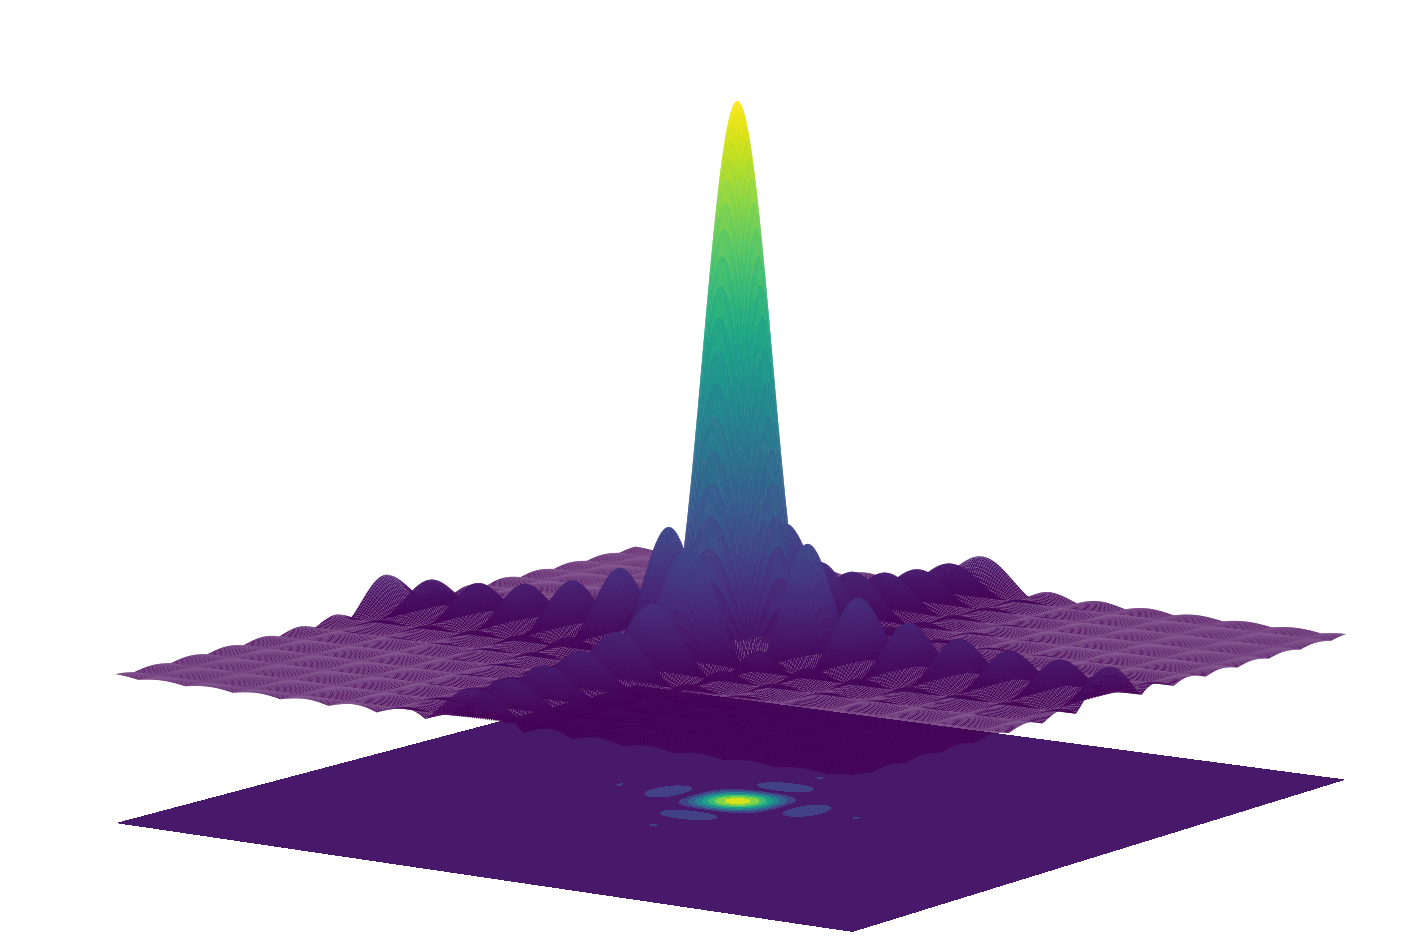
\includegraphics[width = \textwidth]{Figures/Cubic_aperture.png}
		\caption{cubic aperture}
		\label{cubicAperture}
	\end{subfigure}
	\begin{subfigure}{0.5\linewidth}
		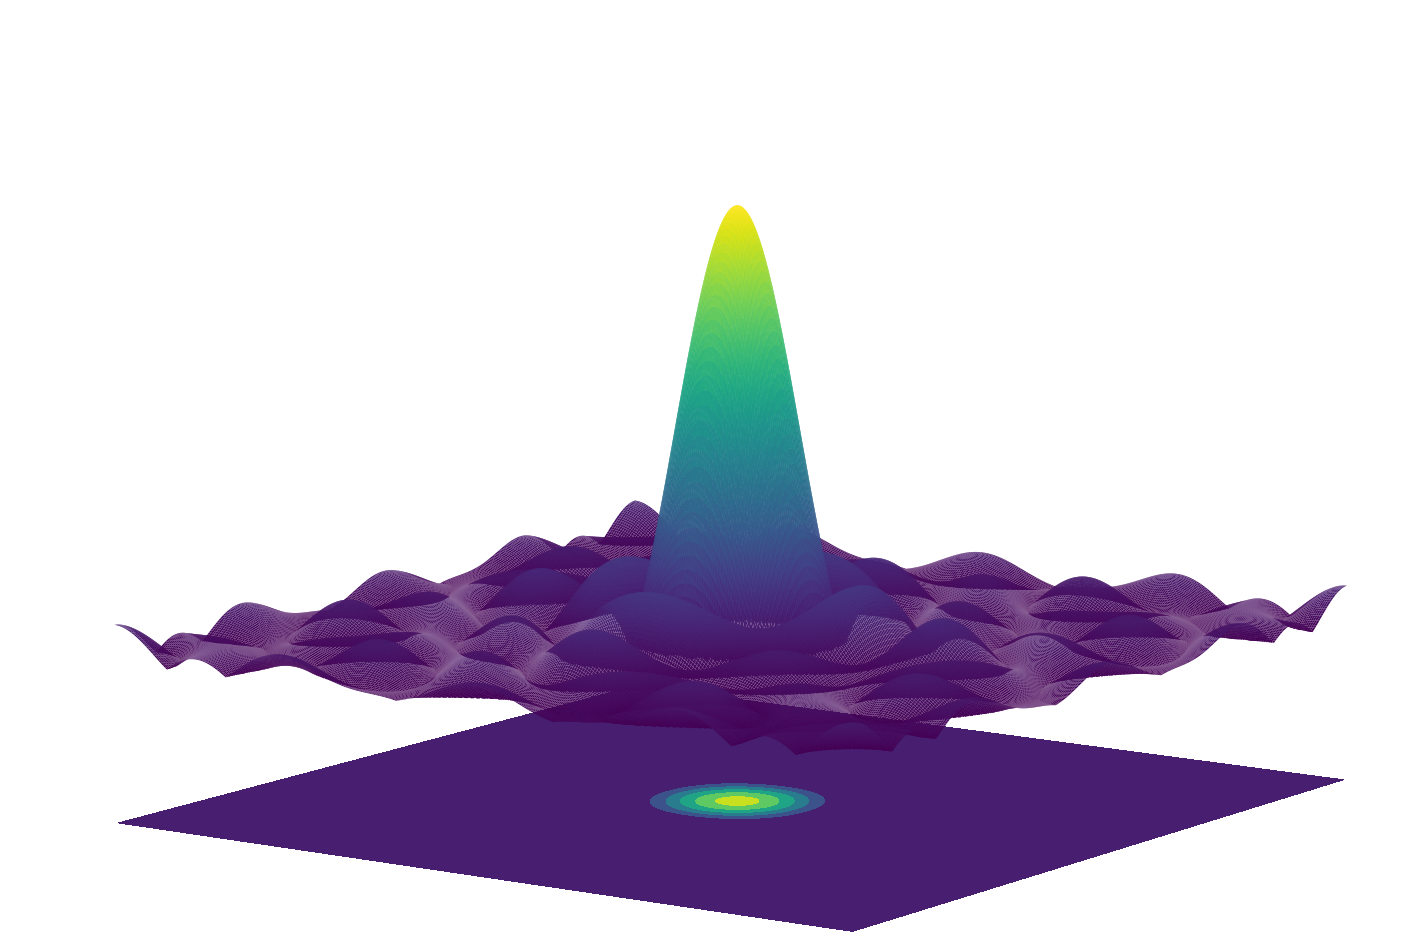
\includegraphics[width = \textwidth]{Figures/Circular_aperture.png}
		\caption{circular aperture}
		\label{circularAperture}
	\end{subfigure}
	\caption{Two figures}
\end{figure}
			\end{lstlisting}
		\end{minipage}
		\column{0.5\textwidth}
		\centering
		\begin{minipage}{0.98\textwidth}
			\begin{figure}
				\frame{
\includegraphics[page = 9, width = 0.8\linewidth]{CodeSnippets/CodeSnippets1}}
			\end{figure}
		\end{minipage}
	\end{columns}
\end{frame}

\begin{frame}[containsverbatim]
	\frametitle{Table of contents, list of figures, list of tables}
	\begin{columns}
		\column{0.5\textwidth}
		\centering
		\begin{minipage}{0.9\textwidth}
			\begin{lstlisting}
\end{titlepage}
\cleardoublepage
% Table of contents stuff
\pagenumbering{roman}
\tableofcontents
% \cleardoublepage
% List of figures, list of tables
\listoffigures
\listoftables

\thispagestyle{empty}
\addcontentsline{toc}{section}{\numberline{}List of Figures}
\addcontentsline{toc}{section}{\numberline{}List of Tables}
\cleardoublepage

% Main body stuff
\pagenumbering{arabic}
\setcounter{page}{1}

\cleardoublepage
\section{Introduction} 
			\end{lstlisting}
		\end{minipage}
		\column{0.5\textwidth}
		\centering
		\begin{minipage}{0.98\textwidth}
			\begin{figure}
				\frame{
\includegraphics[page = 2, width = 0.8\linewidth]{CodeSnippets/CodeSnippets1}}
			\end{figure}
		\end{minipage}
	\end{columns}
\end{frame}

\begin{frame}
	\frametitle{Templates}
	
	We will demonstrate some useful \LaTeX\xspace templates. 
	
	\bigskip
	
	However, keep in mind that before you use templates, you should make yourself comfortable with the basic \LaTeX\xspace commands.
	
\end{frame}

\begin{frame}
\frametitle{The last session: Q and A}

Hopefully, hopefully and hopefully we will be able to answer your questions.

\bigskip

\Huge{Thank you!}

\end{frame}

\end{document}